% !TEX root = ./../../_Thesis.tex

% section's Name and Label
\subsection{Optical Simulation Techniques}
\label{subsec:OpticalSimulationTechniques}

\citet{Barsky2004} proposed a method for generating synthetic images incorporating the optical characteristics of an individual. Specifically, his method simulates the perception of an individual based on data acquired using a Shack-Hartmann wavefront aberrometer. Figure \ref{fig:barsky_algorithm} shows a rendered image using his technique, along with an overview of the algorithm. Note that once the wavefront data is captured, it is sampled to calculate an {\it Object Space PSF} (OSPSF) and used to blur the input synthetic scene at different depths.

\begin{figure}[h]

	\centering
	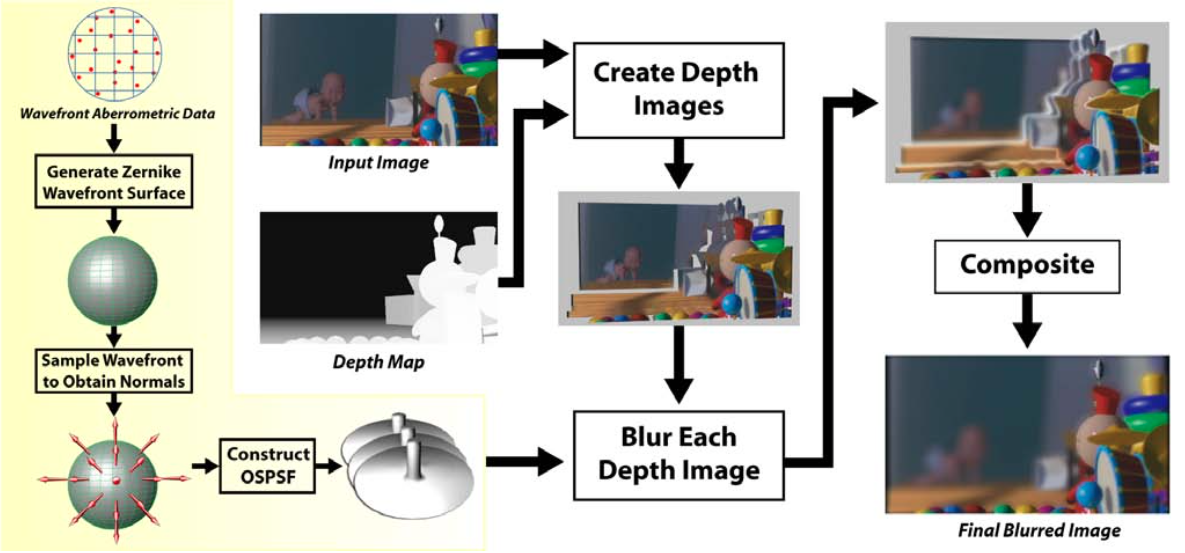
\includegraphics[width=0.99\linewidth]{__Images/03/barsky_pipeline.png}
	\caption[Overview of the vision-realistic rendering algorithm]{Overview of the vision-realistic rendering algorithm proposed by \citet{Barsky2004}. Given an individual's wavefront data and some synthetic scene, one can
	%one can compute the deviation from where the centroids would be in for an ideal wavefront; 
	generate millions of samples necessary to calculate an OSPSF; create a set of depth images; blur each depth image; and composite them to obtain a final blurred image.}
	\label{fig:barsky_algorithm}
\end{figure}

Many researchers have used raytracing techniques and anatomical optics to study and simulate vision by using theoretical models of the human eye \cite{Camp1990, Kolb1995}. \citet{Camp1990} described two ray tracing algorithms for deriving an optical PSF from corneal topography measurements. They focused on simulating and evaluating optical performance of patients' eyes with the following corneal pathologies: \emph{keratoconus}, \emph{epikeratophakia for aphakia} and \emph{radial keratonomy}. \citet{Kolb1995} presented a physically-based camera model that simulates aberration and radiation. To simulate such effects, they compute the geometry of image formation of a particular lens system using a modified distributed ray tracing algorithm. The algorithm is a hybrid of rendering and lens maker techniques, and can produce images of synthetic scenes showing a variety of optical effects. \citet{Mostafawy1997} combined the algorithm presented by \citet{Kolb1995} and the dimensions of an schematic eye model to generate virtual simulations of vision after corrective surgery.

\begin{figure}[!b]
	\centering

	\subfigure[Shack-Hartmann device's output]{
		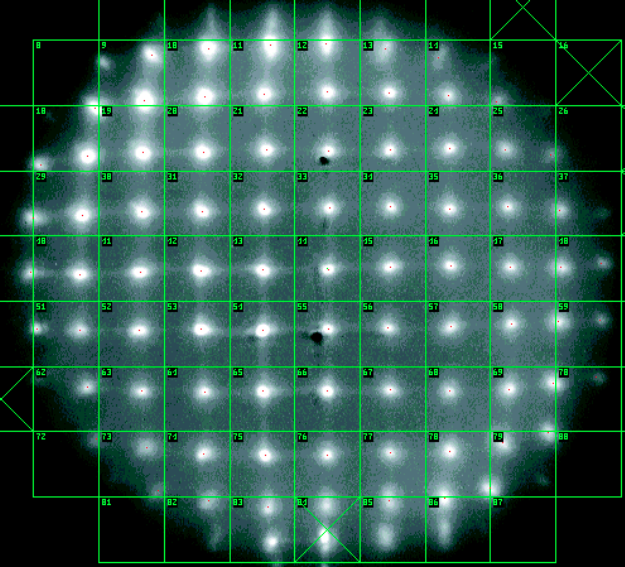
\includegraphics[width=140, height=140]{__Images/03/shackhartmann.png}
		\label{fig:yuA}
	}
	~
	\subfigure[Focused at infinity]{
		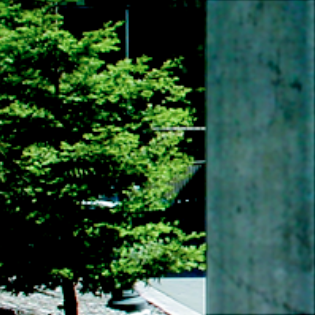
\includegraphics[width=140, height=140]{__Images/03/focused_atInf.png}
		\label{fig:yuB}
	}
	~
	\subfigure[Focused at 0.5m]{
		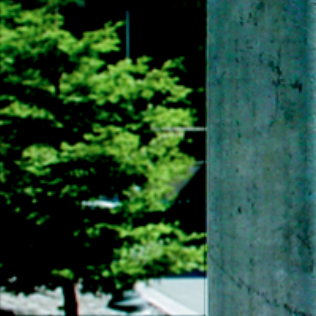
\includegraphics[width=140, height=140]{__Images/03/focused_atX.png}
		\label{fig:yuC}
	}
	
	\caption{\citet{Yu2001} uses data captured using a Shack-Hartmann aberrometer (a) to simulate blur at specific depth values (b) and (c).}
	\label{fig:yu}
\end{figure}

Moreover, the study of monochromatic aberrations of the human eye with wavefront sensors \cite{Liang1994} allowed many others to perform simulations by using Fourier tools to mimic visual perception. \citet{Yu2001} presents a technique capable of generating simulations of synthetic and  real scenes focusing at a specific depth (Figures~\ref{fig:yuB} and \ref{fig:yuC}). Instead of considering only the corneal surface and using raytracing techniques to perform such simulations, the authors rely on data captured by a Shack-Hartmann device (Figure~\ref{fig:yuA}). With this information they construct a wavefront, which is used to blur a sharp image according to a depth map. However, they do not present a proper way of evaluating the simulations' outcomes, which could be, for example, compared with an optical ground truth. 
\citet{Watson2008} proposed an image-based model for predicting acuity from optical aberrations. In this model, a `neural image' is computed incorporating optical and neural filtering. Then, this image is presented to four human observers and the LogMAR acuity is evaluated. By doing this, they can relate visual acuity as a function of a particular aberration and compute predictions of how a specific aberration (\eg, defocus) affects visual acuity.

%\textcolor{red}{NAO BASTA MENCIONAR OS OUTROS TRABALHOS. VOCE PRECISA DEIXAR CLARA AS DIFERENCAS ENTRE O QUE VOCE ESTÁ PROPONDO E O QUE OS OUTROS FIZERAM.}